\documentclass[10pt,A4]{aastex62}
\usepackage{ucs}
%\usepackage{newtxtext,newtxmath}
% Depending on your LaTeX fonts installation, you might get better results with one of these:
%\usepackage{mathptmx}
\usepackage{amsfonts,amssymb,amsmath}
\usepackage{txfonts}
%\usepackage[T1]{fontenc}
\usepackage{graphicx}	% Including figure files
\usepackage{commath}

\usepackage{savesym}
\savesymbol{tablenum}
\usepackage[alsoload=astro]{siunitx}
\restoresymbol{SIX}{tablenum}

\usepackage{hyperref}
\usepackage{bm}
\newcommand{\rvline}{\hspace*{-\arraycolsep}\vline\hspace*{-\arraycolsep}}

\begin{document}
\title{Notes on Abacus BAO Analyses}
\correspondingauthor{Duan Yutong}
\email{dyt@physics.bu.edu}

\author[0000-0002-0786-7307]{Duan Yutong}
\affil{Boston University}

% Abstract of the paper
\begin{abstract}
This serves as detailed notes on the procedures of BAO analysis with AbacusCosmos to accompany the code. Part 1 is on the calculation of correlation functions and covariance matrices. Part 2 is on the fitting methods of the BAO fitter.
\end{abstract}

%%%%%%%%%%%%%%%%%%%%%%%%%%%%%%%%%%%%%%%%%%%%%%%%%%

%%%%%%%%%%%%%%%%% BODY OF PAPER %%%%%%%%%%%%%%%%%%

\section{Introduction}

Precision measurement of the BAO signal from galaxy correlation functions requires understanding the systematics. The standard approach is producing many mock catalogues of galaxies/quasars, test the analysis pipelines, and evaluate the sensitivity to systematics. The pipelines largely consist of two parts, statistics and fitting. The statistics of galaxy catalogues are correlation functions and covariance matrices. Then the statistics are fed to the fitting procedures, yielding best-fit $\alpha$, the BAO scale parameter with respect to the fiducial model.

\section{Correlation Functions and Covariance Matrix}

	\subsection{Reading Halo Catalogue}
		
		Given a cosmology and a redshift, there are 16 boxes with varied phases. For each phase, load the halo catalogue produced by the Rockstar halo-finder. The virial mass and radius fields have inconsistent naming so add the following columns if they are not already present
		\begin{align}
			\mathtt{halo\_mvir} & = \mathtt{halo\_m} \\
			\mathtt{halo\_rvir} & = \mathtt{halo\_r}
		\end{align}
		to keep the Abacus catalogues compatible with halotools, where these fields are assumed to be present. The halo mass field \texttt{halo\_mgrav} is preferred over \texttt{halo\_mvir} in calculations because \texttt{halo\_mvir} only works well for large halos and misbehaves for small halos as well as subhalos. For our analysis the distinction is not important though. 
		
		The NFW profile $\rho(r)$ is a mass distribution model for dark matter halos as a function of radius. The profile is completely characterised by \texttt{halo\_mvir} and the the concentration $c_\text{NFW} \equiv R_\text{vir}/{R_s}$, where $R_s$ is the scale radius of the halo (see \href{http://halotools.readthedocs.io/en/latest/source_notes/empirical_models/phase_space_models/nfw_profile_source_notes.html#nfw-profile-tutorial}{halotools implementation} for formulae). The Klypin definition of the halo scale radius $R_\text{s}$ is considered more stable than the usual $R_\text{s}$ for small halos. The NFW concentration field is added to halo table as well.
		\begin{equation}
			\mathtt{halo\_nfw\_conc} = \frac{\mathtt{halo\_rvir}}{\mathtt{halo\_klypin\_rs}}.
		\end{equation}
		
	\subsection{Halotools Prebuilt HOD Models}
		
		Halotools treats all halos as spherical and uses NFW profiles to paint galaxies. Several mainstream HOD models are built in to halotools: \texttt{['zheng07', 'leauthaud11', 'tinker13', 'hearin15', 'zu\_mandelbaum15', 'zu\_mandelbaum16', 'cacciato09']}. We tune the model parameters to generate LRG-like samples. For a $(\SI{1100}{\mega\parsec/h})^3$ simulation box, typical numbers are
		\begin{align}
			N_\text{halos} & = \num{8e6}\\
			N_\text{galaxies} & = \num{5e5}.
		\end{align}
		The \cite{zheng07} model used in SDSS is an essential model with 5 parameters, $(M_\text{cut}, \sigma, M_0, M_1, \alpha)$. The mean halo occupation numbers per halo for central and satellite galaxies are given by
		\begin{align}
			\left< N_\text{cen} (M) \right> &= \frac{1}{2} \left[ 1 + \mathrm{erf} \left( \frac{\log M - \log M_\text{cut}}{\sigma} \right) \right] \nonumber \\
			&= \frac{1}{2} \mathrm{erfc} \left( \frac{\log(M_\text{cut} / M)}{\sigma} \right) \\
			\left< N_\text{sat} (M) \right> &= \left< N_\text{cen} (M) \right> \left( \frac{M - M_0}{M_1} \right) ^\alpha \, .
		\end{align}
		
	\subsection{Generalised HOD Model}
		
		\subsubsection{Baseline Model (Zheng07 or White11)}
			
			Since Abacus enables direct access to DM particles beyond standard halo metadata, a DM particle-based approach can be used to populate halos, without invoking NFW concentrations. Satellite galaxies are assigned to each DM particle within the halo with a certain probability, such that the resulting mean occupation is as specified by the HOD model. This avoids sphericalising halos and respects the morphology of halos when assigning synthetic galaxies. For the first BOSS analyses \cite{white11} used Zheng's formalism but with slightly different parametrisations,
			\begin{align}
				\left< N_\text{cen} (M) \right> &= \frac{1}{2} \mathrm{erfc} \left( \frac{\ln(M_\text{cut} / M)}{\sqrt{2} \sigma^\prime} \right) \\
				\left< N_\text{sat} (M) \right> &= \left< N_\text{cen} (M) \right> \left( \frac{M - \kappa M _\text{cut} }{M_1} \right) ^\alpha \, .
			\end{align}
			where the argument inside erf has an extra factor of $\ln 10 / \sqrt{2}$, and $M_0$ is replaced with $\kappa M_\text{min}$. The reason for the trivial change of parametrisation was that ``our definition of $\sigma$ can be interpreted as a fractional `scatter' in mass at threshold". Conversion of SDSS/BOSS empirical values to the new parameters $(M_\text{cut}, \sigma^\prime, \kappa, M_1, \alpha)$  can be done simply by
			\begin{align}
				\sigma ^\prime &= \frac{\ln 10}{\sqrt{2}} \sigma \\
				\kappa &= \frac{M_0}{M_\text{min}}
			\end{align}
			with $M_\text{cut}$, $M_1$ and $\alpha$ remaining the same.
			
			The halo table and particle subsample table are loaded with appropriate mass cut applied and subhalos dropped. This selection cut help to remove small halos whose profiles are strongly
			affected by the force softening length, resulting in nonphysical halo profiles.When populating halo catalogues with galaxies, several observational effects are added to the truth so that the data appear realistic. The bias implementation in the generalised HOD model is similar to \cite{yuan2018}.
			
			With 16 phase boxes, to further increase the signal-to-noise in the clustering statistics, 10-16 realisations of a given HOD is generated with different initial seeds for each box. Given a phase $p$ and realisation $r$, the random number generator seed is chosen as
			\begin{equation}
				s = 100p + r
			\end{equation}
			which guarantees that the random numbers only depend on the phase and realisation as we never go beyond 100 realisations. In other words, different HOD models always result in the same random numbers assigned to halo centres and subsample DM particles in a fixed order regardless of any HOD parameters. 

		\subsubsection{RSD for Centrals and Satellites}
		
			Redshift-space distortion seen by an observer is added to simulation by just modifying the $z$-coordinate of the halo/galaxy,
			\begin{align}
				x _z^\prime = x_z + \frac{v_z}{ a H(a) } = x_z + \frac{v_z}{\frac{H(z)}{1+z}} = x_z + \frac{1+z}{H(z)} v_z
			\end{align}
			as derived in \href{http://halotools.readthedocs.io/en/latest/source_notes/mock_observables/zspace_distortions.html}{halotools documentation}. This formula a very good approximation. However, halotools assumes $h=1$ and $H_0=100h = \SI{100}{\kilo\meter\per\second\per\mega\parsec}$, whereas our simulations are more realistic and were run with $h \approx 0.67$, so we are avoiding the Halotools implementation. There are two ways to manually add RSD, bypassing relevant halotools functionalities. One is to use Astropy's cosmology class, which comes as \texttt{halocat.cosmology} and includes the $E$ function $E(z) = \int_{0}^{z} \frac{H_0}{H(z^\prime)} \dif z^\prime$ for the particular cosmology. With $H(z) \equiv H_0 E(z)$, RSD can be implemented as
			\begin{equation}
				x_z ^\prime = x_z + \frac{1+z}{H_0 E(z)} v_z
			\end{equation}
			The other way is to use the conversion factor in halo catalogue header \texttt{halocat.header['VelZSpace\_to\_kms']}, defined as
			\begin{equation}
				\beta \equiv aH(z) L_\text{box} = \frac{H(z)}{1+z} L_\text{box}
			\end{equation}
			where $\beta$ is in \SI{}{\kilo\meter\per\second}  and $L_\text{box}$ in \SI{}{\mega\parsec}. RSD is then applied as
			\begin{equation}
			x_z ^\prime = x_z + \frac{L_\text{box}}{\beta} v_z \, .
			\end{equation}
			where $x_z$ and $v_z$ are in default catalogue units of $\SI{}{\mega\parsec}$ and $\SI{}{\kilo\meter\per\second}$. These two methods are numerically equivalent up to 1 in $10^{15}$.
			
		\subsubsection{Assembly Bias for Centrals (Ranking)}
			
			First all catalogues from 16 phases are loaded with mass cut $4\times 10^{12} M_\odot$ and subhalos dropped, and for 100 log halo mass bins between the minimum and maximum log masses, the median NFW concentration is extracted. With 100 bin centre mvir values in unit of $h^{-1} M_\odot$ and 100 $c_\text{median}$ values, a 3rd order polynomial fit is performed and looks like Fig. \ref{fig:c_median_poly}.
			
			\begin{figure}
				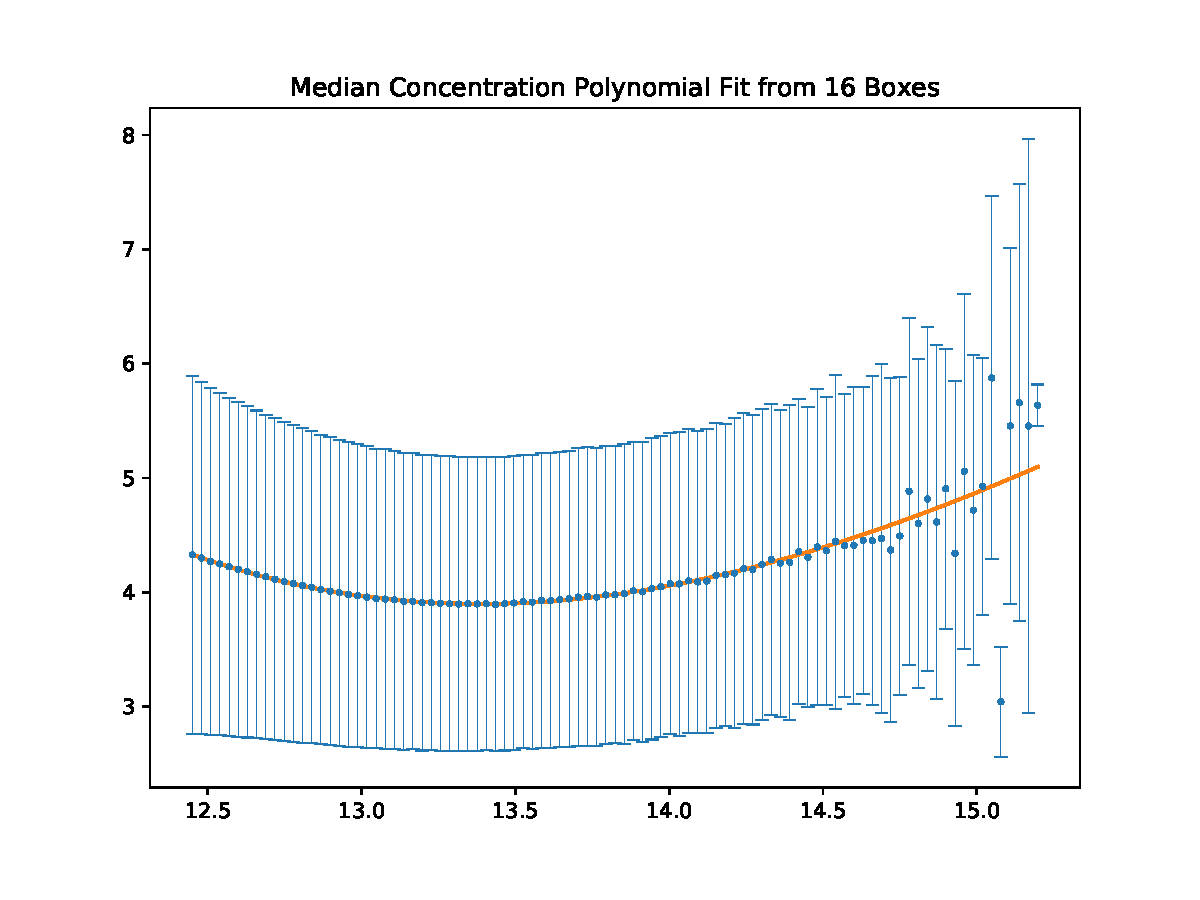
\includegraphics[width=\linewidth]{c_median_poly.pdf}
			    \caption{Median concentration as a function of log halo virial mass.}
			    \label{fig:c_median_poly}
			\end{figure}
			
			Instead of the usual weight $ w = 1/\sigma(c)$ which yields very large weight for bins with very small number of halos and very small standard deviation in $c$, a correction is applied to explicitly weigh the number of halos in the bin
			\begin{equation}
				w = \frac{1}{\sigma(c)}  \sqrt{N_\text{halos} - 1}.
			\end{equation}
			Data are also masked for extremal cases where $N_\text{halos}$ in a bin is only 0 or 1.
			
			Now, with this polynomial fit, we may compare the $c_\text{NFW}$ of any given halo with the $c_\text{median}$ at that halo mass scale of the halo. Define pseudomass of centrals as
			\begin{equation}
				\log M_\text{pseudo} = log M + A_\text{cen} \left[ 2 \Theta(c-c_\text{med}) - 1 \right]
			\end{equation}
			so that when $c > c_\text{med}$ there is a $+A_\text{cen}$ correction, and when $c < c_\text{med}$, $-A_\text{cen}$.
			
			Next the masses and pseudomass are sorted and re-assigned to halos: the halo with highest pseudomass (rank 0 halo) gets the highest actual mass, and so forth. We have not modified any halo mass values, just re-assigned them by pseudomasses. The new halo masses are used as input for HOD models and calculating theoretical mean occupation $\left<N_\text{cen}\right>$, and never written to the original halo table.
			
		\subsubsection{Velocity Bias for Centrals}
		
			The velocity bias for central galaxies is added by randomly drawing the peculiar velocity from a normal distribution corresponding to the RMS dispersion within the halo,
			\begin{align}
				v_\text{pec} &\sim N(0, \frac{v_\text{rms}}{\sqrt{3}} \alpha_c) \\
				v_\text{los} ^\prime &= v_\text{los} + v_\text{pec}
			\end{align}
			assuming $v_\text{rms} = \sqrt{v_x^2 + v_y^2 + v_z^2}$ and $v_\text{los} = v_z$.
			
		\subsubsection{Assembly Bias for Satellites (Ranking)}
			
			The assembly bias for satellites is completely independent from that for centrals, and either can be turned on or off. The original halo masses are read from halo table again, and re-assigned using pseudomass
			\begin{equation}
				\log M_\text{pseudo} = log M + A_\text{sat} \left[ 2 \Theta(c-c_\text{med}) - 1 \right]
			\end{equation}
			and the HOD models take new masses as input and produce $\left<N_\text{sat}\right>(M)$. No particle property is involved here and $\overline{p} = \left< N_\text{sat} \right> / N_\text{part}$ is the same for all particles in the same halo.
			
		\subsubsection{Host Centric Distance Ranking for Satellites}
			
			The probability of a particle hosting a satellite straight from an HOD model $\overline{p} = \left<N_\text{sat}\right> / N_\text{part}$ is modified by several ranking procedures. The first is ranking by host centric distance, i.e. the distance between the particle and halo centre. The furthest particle gets rank $r_i=0$, and so forth. With a constant modulation parameter $s$ specified, the probability is modified as
			\begin{equation}
				p_i = \overline{p} \left[ 1 + s (1 - \frac{2 r_i}{N_\text{part} - 1}) \right] .
			\end{equation}
			
		\subsubsection{Velocity Bias for Satellites (Ranking)}
			
			The second particle ranking procedure adds velocity bias for satellites. The peculiar speed of each halo particle is calculated, and within each halo, the particles are ranked by their peculiar speed: particle with highest peculiar speed has rank $r_i=0$. The probability then becomes
			\begin{equation}
				p_i ^\prime = p_i \left[ 1 + s_v (1 - \frac{2 r_i}{N_\text{part} - 1}) \right] .
			\end{equation}
			
		\subsubsection{Perihelion Distance Ranking for Satellites}
			
			The last particle ranking procedure ranks particles by their distance of closest approach to halo centre. The perihelion distance $r_\text{min}$ is numerically approximated with an iterative approach (\cite{yuan2018}), which takes ~10 iterations for average fractional error to reach 10\% and ~30 iterations for the maximum fractional error to drop below 10\%. Particle with the largest $r_\text{min}$ gets rank $r_i = 0$. Then again
			\begin{equation}
				p_i ^\prime = p_i \left[ 1 + s_p (1 - \frac{2 r_i}{N_\text{part} - 1}) \right] .
			\end{equation}
			
		Finally, each particle gets a random number between 0 and 1, and those below the theoretical $p_i$ get satellites. Even when the HOD models give negative probabilities, this will not misbehave. For each realisation of each HOD model in each phase box, the galaxy table is saved as in astropy ASCII csv format.

	\subsection{Galaxy Pair Counting}
	
		All counting is done in fine $(s, \mu)$ bins: $s$ bin edges are from 0 to \SI{150}{h \tothe{-1} \mega\parsec} at \SI{1}{h \tothe{-1} \mega\parsec} steps, and $\mu \equiv \cos\theta$ bin edges are from 0 to 1 at 0.01 steps, meaning a total of $(150, 100)$ bins.
		
		We need the auto-counts for each box to calculate the auto-correlation for the whole box, and the cross-counts between the box and a subvolume of itself to calculate cross-correlation and estimate the covariance matrix. All these counts are saved to disk. Raw counts are saved as \texttt{paircount-DD.npy} in the original Currfunc count format, i.e. a structured array. Note that \texttt{c\_api\_timer} needs to be turned off in Corrfunc for this file to be saved and recovered properly and not as ``object'' type. 
		
		The optimal $s$ bin size and range for fitting were studied in BOSS DR12 analysis \cite{boss_dr12_bao}. Based on these results, we choose the bin	size \SI{5}{h \tothe{-1} \mega\parsec} and the range $\SI{50}{h \tothe{-1} \mega\parsec} < s < \SI{150}{h \tothe{-1} \mega\parsec}$. Also we use a $\mu$ bin size of 0.05 to be consistent with BOSS DR12. The raw counts were re-binned into $(30, 20)$ coarse bins and total pair counts verified.
		
	\subsection{Auto-correlation Functions}
		
		The PH natural estimator of the auto-correlation requires $DD$ and $RR$ counts for each phase box. $DD$ is calculated using the re-binned DD counts for $(30, 20)$ bins. $RR$ pair counts are calculated for the same bins analytically as given in Appendix \ref{appendix_auto_correlation}.
		
		The auto-correlation function $\xi$ is decomposed into the monopole component $\xi_0$ for $\ell=0$ and the quadrupole component $\xi_2$ for $\ell=2$ in the Legendre spherical harmonics basis using
		\begin{align}
			\xi (s, \mu) 	&= \sum_{\ell} \xi_\ell (s) P_\ell(\mu) \\
			\xi _\ell (s) 	&= \frac{2\ell + 1}{2} \int_{-1}^{1} \xi(s, \mu) P_\ell (\mu) \dif \mu \label{eqn:xi_decomp}
		\end{align}
		as shown in Fig. \ref{fig:xi_r10_phases}. If
		clustering were perfectly isotropic, the $\ell > 0$ moments would all be zero. Anisotropy introduces power into the even-order multipoles;
		however, the odd-order multipoles are always zero due to symmetry. 16 $\xi$ samples from 16 realisations are averaged and become a single auto-correlation result for the box. This averaging step can be done before or after multipole decomposition which is a linear operation.
		
		\begin{figure}
			% To include a figure from a file named example.*
			% Allowable file formats are eps or ps if compiling using latex
			% or pdf, png, jpg if compiling using pdflatex
			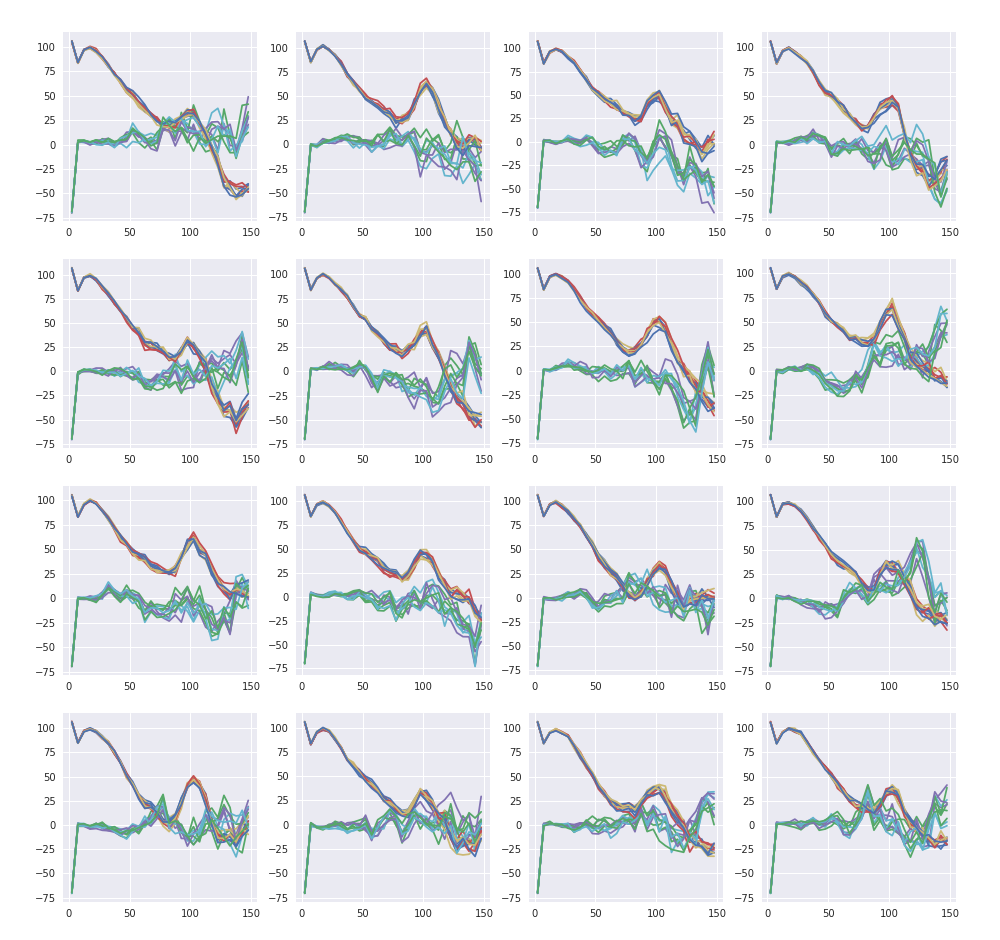
\includegraphics[width=\linewidth]{xi_r10_phases_tinker13.png}
		    \caption{Monopole and quadrupole of auto-correlation functions for 16 phase boxes. Each box has 16 realisations overplotted, which are averaged to give one result.}
		    \label{fig:xi_r10_phases}
		\end{figure}
		
		Then we jackknife co-add the 16 boxes, dropping one box at a time and taking the mean of the other 15. This yields 16 jackknife correlation function samples, and each one is passed on to the fitter for BAO fitting.
		
		To be consistent with FFT correlation code, BAo analysis has switched to the Landy \& Szalay (1993) estimator defined in Appendix \ref{appendix_LS}.

	\subsection{Covariance Matrix}
		
		The BAO fitter takes correlation functions and covariance matrix as input. The covariance is empirically estimated. Each simulation box is divided into $N_\text{sub}^3=3^3$ subvolumes. The cross-correlation function between one subvolume and the entire box is calculated for all 16 phases, resulting in $27 \times 16 = 432$ correlation function samples if there is only 1 realisation. For 10 realisations there would be 4320 samples, from which covariance between every two bins are calculated. With 30 $s$ bins for multipole data $\xi_0$ and $\xi_2$, there are $30\times 2 = 60$ bins, monopole and quadrupole included. The resulting covariance matrix has dimension $60\times 60$.
		
		Finally this covariance matrix needs to be rescaled before fitting to account for the survey volume, as the $\xi$ data are derived from $V_\text{box} = (\SI{1100}{\mega\parsec/h})^3 $. The covariance scales inversely with volume, so the covariance derived from the subvolume ($1/27$ of the box's volume) is 27 times the actual, hence a factor of $1/27$. Realisations of HOD models can be treated as independent mocks, like the 16 independent phase boxes. 
		
		Due to the delete-1 jackknife procedure applied to $\xi$ samples, which are the average of 15 boxes, the scatter in the fitted $\alpha$ values are underestimating the uncertainty in $\alpha$ for the given HOD model. We take the standard deviation in $\alpha$ multiplied by $\sqrt{15}$ as the uncertainty in $\alpha$.
		
\section{BAO Fitting Methods}

	\subsection{BOSS DR12 Fitter}

		A recent, functional \href{https://github.com/ashleyjross/LSSanalysis} {fitter} by Ross was used for BOSS DR12 analysis (\cite{boss_dr12_bao}). The fitter takes correlation function data $\xi_0, \xi_2$ in all $(s,\mu)$ bins and the covariance between all bins as input, and evaluates $\chi^2$ in the $(\alpha_\varparallel, \alpha_\perp)$ parameter grid. Theoretically, from Eqn. \ref{eqn:xi_decomp} we have
		\begin{align}
			\xi_0 (r)
				&= \frac{1}{2} \int_{-1}^{1} \xi(r, \mu) P_0(\mu) \dif \mu 
				= \int_{0}^{1} \xi(r, \mu) \dif \mu \\
			\xi_2 (r)
				&= \frac{5}{2} \int_{-1}^{1} \xi(r, \mu) \frac{1}{2} (3\mu^2 - 1) \dif \mu \\
				&= 5 \left[ \int_{0}^{1} \frac{3}{2} \mu^2 \xi(r, \mu) \dif \mu -\frac{1}{2} \xi_0 (r) \right]\\
				&= 5 \left[ \xi_{\mu 2} (r) - \frac{1}{2} \xi_0 (r) \right]
		\end{align}
		where we have used the even properties of even $P_\ell(\mu)$ and defined a shorthand $\xi_{\mu 2} (r)$. Therefore the model for fitting the $(\xi_0, \xi_2)$ data is chosen as
		\begin{align}
			\xi _0^\text{fit} (r) &= B_0 \xi_0^\text{mod}(r) + \left( A_{00} + \frac{A_{01}}{r} + \frac{A_{02}}{r^2} \right) \label{eqn:xi_0_fit}\\
			\xi _2^\text{fit} (r) &= 5 \left[ B_2 \xi_{\mu 2}^\text{mod} (r) - \frac{B_0}{2} \xi_0^\text{mod}  (r) \right] + \left( A_{20} + \frac{A_{21}}{r} + \frac{A_{22}}{r^2} \right) \label{eqn:xi_2_fit}
		\end{align}
		where $\xi_0^\text{mod} (r), \xi_2^\text{mod} (r)$ are calculated from the template.
		The work flow is detailed as follows.
		
		\renewcommand{\labelenumi}{(\Roman{enumi})}
		\begin{enumerate}
		
			\item 
			A template $\xi^\text{fid}_\ell(r)$ is generated beforehand for $\ell = 0,2,4$ using the linear power spectrum $P_\text{lin}(k)$ from {\scshape{Camb}} for $r=10$ to $ \SI{299}{\mega\parsec/h}$ with spacing 1 in the fiducial cosmology. A ``no-wiggle'' template is available but not actually used in the fitting.
			
			\item 
			Input $\xi$ and covariance data are masked according to the proper $r$ range for fitting, $50$ to $\SI{150}{\mega\parsec/h}$, and $N=20$ bins are selected. Also a prior/bias model takes the data within $50$ to $ \SI{80}{\mega\parsec/h}$, $N^\text{bias} = 6$. The data vector $\bm{\xi} = (\bm{\xi}_0, \bm{\xi}_2) ^T$ is a $2N \times 1$ vector. The reduced-size covariance matrix containing appropriate bins is inverted and taken as the precision matrix, $C^{-1} (2N \times 2N)$ and $C_\text{bias}^{-1} (2N^\text{bias} \times 2N^\text{bias})$. Grid search $\alpha$ range and spacing are also specified.
			
			\item 
			First the bias model is analysed, without using any observed data. Set $\alpha_\varparallel = \alpha_\perp = 1, B_0 = B_2 = 1$. For $r$ bin centre data given to the prior model, define
			\begin{align}
				& r^\prime = r \sqrt{\mu^2 \alpha_\varparallel^2 + (1-\mu^2)\alpha_\perp^2} = r\gamma \\
				& \mu^\prime = \frac{\mu \alpha_\varparallel}{\sqrt{\mu^2 \alpha_\varparallel^2 + (1-\mu^2)\alpha_\perp^2}} = \frac{\mu \alpha_\varparallel}{\gamma}
			\end{align}
			and the $\alpha$-rescaled $\xi$ are calculated using fiducial template $\xi^\text{fid}_\ell (r)$,
			\begin{align}
				\xi^\text{mod}_0 (r) &= \int_{0}^{1} \xi^\text{fid}(r^\prime, \mu^\prime) \dif \mu \nonumber \\
					&= \int_{0}^{1} \sum_{\ell=0,2,4} \xi^\text{fid}_\ell (r^\prime) P_\ell( \mu^\prime) \dif \mu \nonumber \\
					&= \int_{0}^{1} \sum_{\ell=0,2,4} \xi^\text{fid}_\ell (r\gamma) P_\ell(\frac{\mu\alpha_\varparallel}{\gamma}) \dif \mu \label{eqn:xi_0_mod}\\
				\xi^\text{mod}_{\mu2} (r) &= \frac{3}{2} \int_{0}^{1} \xi^\text{fid} (r^\prime, \mu^\prime) \mu^2 \dif \mu \nonumber \\
					&= \frac{3}{2} \int_{0}^{1} \sum_{\ell=0,2,4} \xi^\text{fid}_\ell (r\gamma) P_\ell(\frac{\mu\alpha_\varparallel}{\gamma}) \mu^2 \dif \mu \label{eqn:xi_2_mod}. 
			\end{align}
			These are what the fiducial $\xi$ template \textbf{would} look like in $r$ coordinate assuming the $(\alpha_\varparallel, \alpha_\perp)$ rescaling. Note the code has different choice of constants from what's written in the DR12 paper, but both are self-consistent...
			
			Then $\chi^2$ is evaluated for varying $B^\text{bias}_0 \in [0.1, 2)$, while all other parameters are held constant, i.e. $B_2=1$, $\bm{A} = (\bm{A}_0, \bm{A}_2)^T = (0, 0, 0, 0, 0, 0)^T$. $ \xi^\text{mod} _0 (r)$ and $\xi^\text{mod} _2 (r)$ are calculated by plugging Eqn. \ref{eqn:xi_0_mod}, \ref{eqn:xi_2_mod} into Eqn. \ref{eqn:xi_0_fit}, \ref{eqn:xi_2_fit}, and compared to data to obtain $\chi^2$,
			\begin{equation}
				\chi^2 (B_0) = (\bm{\xi} - \bm{\xi}^\text{fit})^\text{T} C^{-1} (\bm{\xi} - \bm{\xi}^\text{fit}) + \left( \frac{\ln(B_0/1)}{100} \right) ^2
				+ \left( \frac{\ln(1/1)}{100} \right) ^2 .
			\end{equation}
			The best-fit $\hat{B}^\text{bias}_0$ which minimises $\chi^2$ is used for fitting data.
			
			\item 
			Now the data are fit by brute force scanning all points all points in the $(\alpha_\varparallel, \alpha_\perp)$ grid and evaluating the $\chi^2$ everywhere. At a given $(\alpha_\varparallel, \alpha_\perp)$ point, $\bm{\xi}^\text{mod}$ is calculated using Eqn. \ref{eqn:xi_0_mod}, \ref{eqn:xi_2_mod}. Now, to marginalise over nuisance parameters $\bm{A}$, the fitting form is manipulated by rearranging terms in Eqn. \ref{eqn:xi_0_fit}, \ref{eqn:xi_2_fit} and considering only the polynomial components of the data,
			\begin{align}
				& \xi_0^\text{ply} (r) \equiv \xi _0^\text{fit} (r) - B_0 \xi_0^\text{mod}(r) =  A_{00} + \frac{A_{01}}{r} + \frac{A_{02}}{r^2} \\
				& \xi_2^\text{ply} (r) \equiv \xi _2^\text{fit} (r) - 5 \left[ B_2 \xi_{\mu 2}^\text{mod} (r) - \frac{B_0}{2} \xi_0^\text{mod}  (r) \right] = A_{20} + \frac{A_{21}}{r} + \frac{A_{22}}{r^2} .
			\end{align}
			making it possible to isolate and analytically find the best-fit nuisance parameters $\bm{A}$ in a linearised fitting model. The $\bm{\xi} ^\text{ply} (r) \equiv (\bm{\xi_0}^\text{ply}, \bm{\xi_2}^\text{ply} )^T$ data are obtained by plugging in $\xi_0, \xi_2$ in place of $\xi_0^\text{fit}, \xi_2^\text{fit}$ above. Define an axillary polynomial matrix
			\begin{equation}
				H^T (r) \equiv 
				\left[
					\begin{array}{c|c}
						\begin{matrix}
							1	& \frac{1}{r}	& \frac{1}{r^2} \\
								& \vdots		& \\
							1	& \frac{1}{r}	& \frac{1}{r^2} 
						\end{matrix}
							& \\
						\hline
					  	&
							\begin{matrix}
								1	& \frac{1}{r}	& \frac{1}{r^2} \\
									& \vdots		& \\
								1	& \frac{1}{r}	& \frac{1}{r^2} 
							\end{matrix}
					\end{array}
				\right]
			\end{equation}
			of dimension $2N \times 6$ with the empty diagonal blocks being all zeros. The fitting model for the polynomial contribution then can be succinctly written as
			\begin{equation}
				\bm{\xi} ^\text{ply} (r) = H^T \bm{A} .
			\end{equation}
			Now minimise $\chi^2$,
			\begin{equation}
				\chi^2 = (\bm{\xi_0}^\text{ply} - H^T \bm{A}) ^T C^{-1} (\bm{\xi}_0^\text{ply} - H^T \bm{A})
			\end{equation}
			and taking $\frac{\partial \chi^2}{\partial \bm{A}} = 0$ yields the normal equation and the analytic solution
			\begin{align}
				H C^{-1} (\bm{\xi}^\text{ply} - H^T \hat{\bm{A}} ) &= 0 \\
				\hat{\bm{A}} &= (HC^{-1}H^T) ^{-1} HC^{-1} \bm{\xi} ^\text{ply}
			\end{align}
			With closed-form $\hat{\bm{A}}$, we may now marginalise over $\hat{\bm{A}}$ and only optimise for $(B_0, B_2)$. $\bm{\xi}^\text{fit}(r)$ is calculated again using Eqn. \ref{eqn:xi_0_fit}, \ref{eqn:xi_2_fit}, and $\chi^2 (B_0, B_2)$ calculated again as
			\begin{align}
				&\chi^2 (B_0, B_2) = \frac{998-2N}{999} \nonumber \\
				&\times \left[ (\bm{\xi} - \bm{\xi}^\text{fit})^\text{T} C^{-1} (\bm{\xi} - \bm{\xi}^\text{fit}) + \left( \frac{\ln(B_0/\hat{B}_0^\text{bias})}{0.4} \right) ^2
				+ \left( \frac{\ln(B_2/\hat{B}_0^\text{bias})}{0.4} \right) ^2 \right]
			\end{align}
			and minimised to find $(\hat{B_0}, \hat{B_2})$. $B_0$ and $B_2$ are required to be non-negative, otherwise $\chi^2=1000$ is returned. The corresponding $\chi^2 (\hat{B}_0, \hat{B}_2) \vline _{(\alpha_\varparallel, \alpha_\perp)}$ is saved and becomes a point in the $\chi^2 (\alpha_\varparallel, \alpha_\perp)$ grid.
		\end{enumerate}
		
		We will write a new fitter in the modern style conforming to PEP standards and optimised for performance.
		
	\subsection{Fitting Results}
	
		The log likelihood ratio follows a $\chi^2$ distribution. In the $\chi^2 (\alpha_\varparallel, \alpha_\perp)$ two-parameter plane, we may find the confidence region for any confidence level $\sigma$ by calculating the constant $\Delta\chi^2$ contour around the minimum $\chi^2$ position. The probability corresponding to confidence level $\sigma$ is
		\begin{equation}
			P = \mathrm{Erf} ( \frac{\sigma}{\sqrt{2}} )
		\end{equation}
		and the contour can be found by
		\begin{equation}
			\Delta \chi^2 = Q(P)
		\end{equation}
		where $Q$ is the quantile function (percent-point function) for a $\chi^2$ distribution with $\mathrm{dof}=2$.
		
		With 16 jackknife $\xi$ samples and a covariance matrix for each HOD model, we obtain 16 best-fit $ (\hat{\alpha}_\varparallel, \hat{\alpha}_\perp) $ points by locating the global $\chi^2$ minimum. Then for every pair of HOD models $M_i$ and $M_j$, we calculate 16 phase-matched differences $\hat{\alpha}_{ij} = \hat{\alpha}_i - \hat{\alpha}_j$, plotted in Fig. \ref{fig:alpha_hod_compare}.
		
		\begin{figure}
			% To include a figure from a file named example.*
			% Allowable file formats are eps or ps if compiling using latex
			% or pdf, png, jpg if compiling using pdflatex
			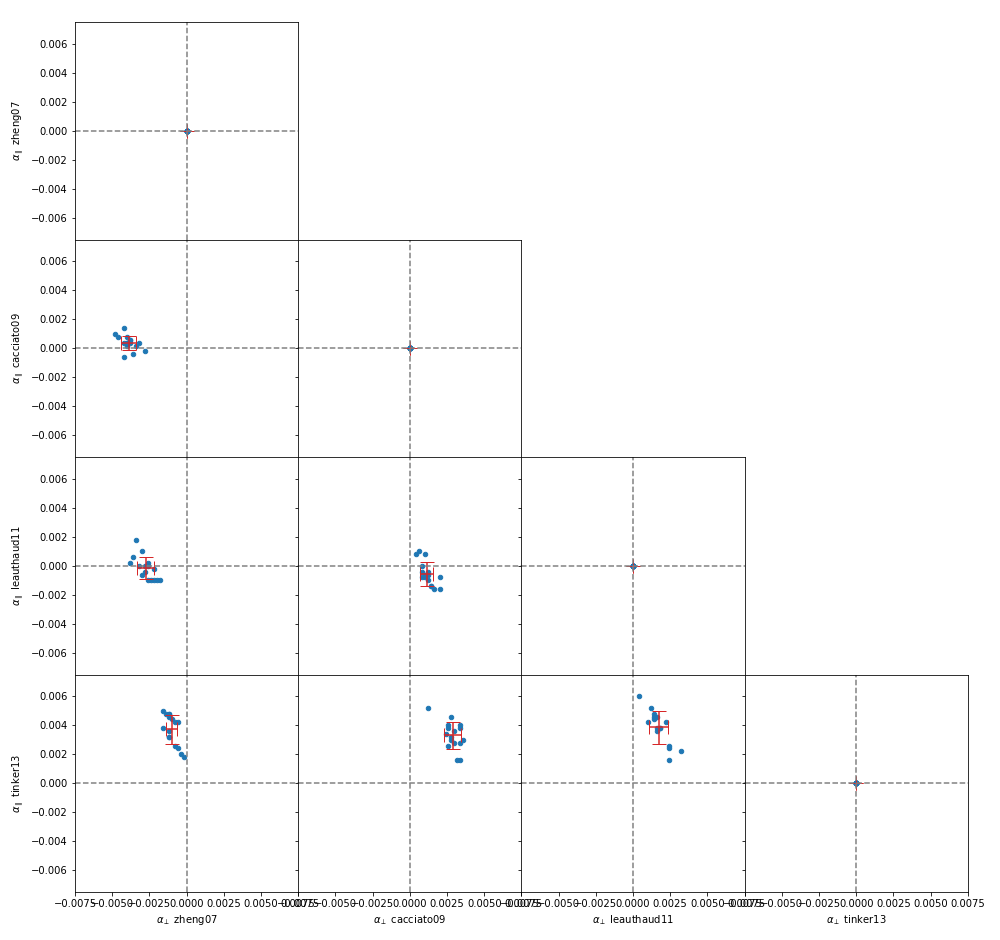
\includegraphics[width=\linewidth]{alpha_pair_compare.png}
		    \caption{Comparison of $ (\alpha_\varparallel, \alpha_\perp) $ for four HOD models done in halotools. vertical axis is $\alpha_\varparallel$, horizontal $\alpha_\perp$. }
		    \label{fig:alpha_hod_compare}
		\end{figure}
		
%%%%%%%%%%%%%%%%%%%%%%%%%%%%%%%%%%%%%%%%%%%%%%%%%%

%%%%%%%%%%%%%%%%%%%% REFERENCES %%%%%%%%%%%%%%%%%%

% The best way to enter references is to use BibTeX:
%\bibliographystyle{abbrv}
\bibliography{ref} % if your bibtex file is called example.bib

%%%%%%%%%%%%%%%%%%%%%%%%%%%%%%%%%%%%%%%%%%%%%%%%%%

%%%%%%%%%%%%%%%%% APPENDICES %%%%%%%%%%%%%%%%%%%%%

\appendix

\section{Auto-correlation Function Estimator}
	\label{appendix_auto_correlation}
	
	In this implementation, raw pair counts are saved, and $N_\text{D}, N_\text{R}$ normalisation is done only at the estimator step.
	
	For auto-correlation of a sample in periodic box, the Peebles \& Hauser (1974) estimator (natural estimator) is
	\begin{equation}
		\xi = \frac{N_\mathrm{R}(N_\mathrm{R}-1)}{N_\mathrm{D}(N_\mathrm{D}-1)} \frac{DD}{RR} - 1
	\end{equation}
	where $DD$ is the auto-correlation data-data pair count and $RR$ is the random-random pair count.
	
	One way to obtain $RR$ is to generate a random sample of particle number $N_\text{R}$ in the same volume and calculate its auto-correlation pair counts. Alternatively, $RR$ can be calculated analytically as follows. Let $\dif V$ be the volume of the $(s, \mu)$ bin and $V=L_\text{box}^3$ be the volume the data sample occupies. The random sample must have the same number density as the data sample, $n_\text{R} = n_\text{D}$. For simple survey geometry, such as a cube, we may well let the random sample have the same number count, volume, and number density as the data sample.
	\begin{equation}
		RR(s, \mu) = \frac{N_\mathrm{R}(N_\mathrm{R}-1)}{V} \dif V(s, \mu)
	\end{equation}
	where $\dif V(s, \mu)$ is the volume of the $(s, \mu)$ bin.
	
\section{Cross-correlation Function Estimator}
	\label{appendix_cross_correlation}
	
	For cross-correlation between a sample $D_1$ in the periodic simulation box and a subsample $D_2$ in its subvolume, the Davis \& Peebles (1983) estimator is
	\begin{equation}
		\xi = \frac{\bar{n}_\text{R1}}{\bar{n}_\text{D1}} \frac{D_1 D_2}{R_1 D_2} - 1
	\end{equation}
	where $\bar{n}_\text{D1}$ is the mean number density of data sample $D_1$, $\bar{n}_\text{R1}$ is the mean number density of $R_1$, the random sample corresponding to $D_1$, $D_1 D_2$ is the cross-correlation pair count between two data samples, and $R_1 D_2$ is the cross-correlation pair count between a random and a data sample. Usually a random sample is about 7 times the size of the corresponding data sample \cite{2008ApJ...687..919W}.

	Again one may generate a random sample $R_1$ in the same volume and do the cross counting, or alternatively calculate it analytically,
	\begin{equation}
		R_1 D_2 = \frac{N_\text{R1} N_\text{D2}}{V_1} \dif V(s, \mu) = \bar{n}_\text{R1} N_\text{D2} \dif V(s, \mu).
	\end{equation}

\section{LS Estimator}
	\label{appendix_LS}

	We use a generalised form of the Landy \& Szalay (1993) estimator to calculate auto- and cross-correlation functions. Given data samples $D_1, D_2$ and random samples $R_1, R_2$ with sample sizes $N_{D1}, N_{D2}, N_{R1}, N_{R2}$, the correlation as a function of pair-counts is
	\begin{align}
		\xi &= \frac{\dfrac{D_1D_2}{N_{D1}N_{D2}} - \dfrac{D_1R_2}{N_{D1}N_{R2}} - \dfrac{R_1D_2}{N_{R1}N_{D2}} + \dfrac{R_1R_2}{N_{R1}N_{R2}}}{\dfrac{R_1R_2}{N_{R1}N_{R2}}} \\
			&= \frac{\overline{DD} - \overline{DR} - \overline{RD} + \overline{RR}}{\overline{RR}}
	\end{align}
	where overline means normalised by sample population sizes, i.e. each pair-count is weighted by $1/N_1N_2$. For auto-correlation, we may simply set $D_1 = D_2$ and $R_1 = R_2$.
	
\end{document}
